\chapter{Indledning}

% Note om hvad der skal stå i dette afsnit her.

\lipsum

\lipsum

\section{Kravspecifikation}

Vi har valgt at lave en plotter, som skal opfylde følgende specifikationer:
\begin{itemize}
\item Plotteren skal kunne tegne noget, som vi har tegnet på computer
\begin{itemize}
\item Skal kunne tegne på et stykke A4-papir
\item Fungere uden at en computern er tilsluttet, læse data fra SD-kort
\end{itemize}
\item Bruge en pen til at tegne
%\begin{itemize}
%\item Bemærk at der ikke skal benyttes blyant eller kuglepen
%\end{itemize}
\item Styre hastigheden af pennen meget præcist
\begin{itemize}
\item Med software skal vi gøre optimalt nytte af stepmotorenes præcision
\end{itemize}
\item Kunne lave nødstop og restart med knapper
%\item Vise status af tegneforløb på LCD-display eller med lysdioder
\item Kunne gå i nulstillingsposition (et sted hvor maskinen ved den så er) ved tryk på en trykknap
\item Kunne glide ligesom vist på figur \vref{fig:plotterskitse}
\mnote{
  % her bør bre$  $dden ikke ændres
  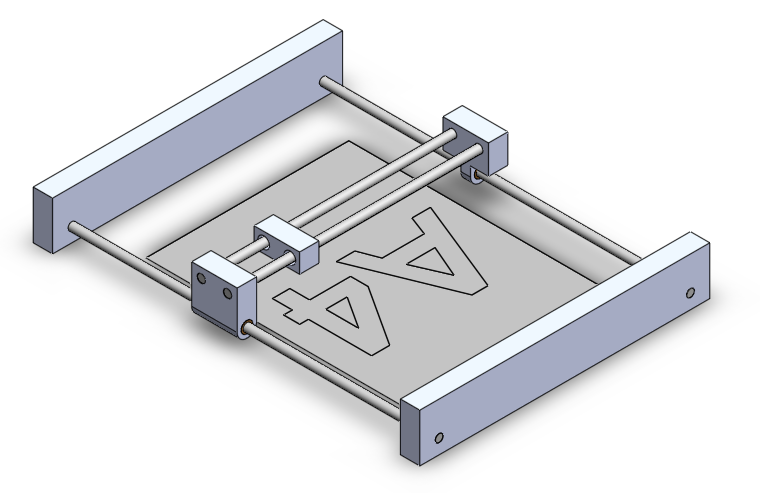
\includegraphics[width=\marginparwidth]{./img/plotterskitse}
  \captionof{figure}{Skitse af konstruktion}
  \label{fig:plotterskitse}
}
\item Bruge tandrem til at trække x- og y-akserne
\begin{itemize}
\item Tandrem er forbundet med stepmotor
\end{itemize}
\item Pennen skulle kunne løftes på tidspunkter, hvor der ikke skal tegnes
\item Kunne implementere rette linjer og cirkler fra HPGL
\end{itemize}



%%% Local Variables: 
%%% mode: latex
%%% TeX-master: "../master"
%%% End: 